\chapter{РК1}

\section{Задание 2}


\textbf{Типы задания:}

1. \textbf{Замыкание.}

Отношение:

R(A,B,C,D,E,F)

Заданы функциональные зависимости:

S = \{

A --> BC,

AC --> DE,

D --> F,

E --> AB

\}

Найти замыкание \{A\}+

\begin{table}[ht]
	\centering
	\begin{tabular}{ | l | l | l |}
		\hline
		ФЗ / Этап & A                & A, B, C, D, E, F \\ \hline
		A --> BC  & A, B, C          & A, B, C, D, E, F \\ \hline
		AC --> DE & A, B, C, D, E    & A, B, C, D, E, F \\ \hline
		D --> F   & A, B, C, D, E, F & A, B, C, D, E, F \\ \hline
		E --> AB  & A, B, C, D, E, F & A, B, C, D, E, F \\ \hline
		\hline
	\end{tabular}
	\caption{Таблица}
	\label{fig:ref11}
\end{table}

Решение: Таблица \ref{fig:ref11}.

Ответ \{A\}+ = \{A, B, C, D, E, F\}

Отношение:

R(A,B,C,D,E,F)

Заданы функциональные зависимости:

R(A,B,C,D,E,F)

S = \{

A --> BC,

E --> CF,

B --> E,

CD --> EF

\}

Найти: \{A, B\}+ ?

Решение: Таблица \ref{fig:ref12}.


\begin{table}[ht]
	\centering
	\begin{tabular}{ | l | l | l | l |}
		\hline
		ФЗ / Этап & A, B       & A, B, C, E    & A, B, C, E, F \\  \hline
		A --> BC  & A, B, C    & A, B, C, E    & A, B, C, E, F \\ \hline
		E --> CF  & A, B, C    & A, B, C, E, F & A, B, C, E, F \\ \hline
		B --> E   & A, B, C, E & A, B, C, E, F & A, B, C, E, F \\ \hline
		CD --> EF & A, B, C, E & A, B, C, E, F & A, B, C, E, F \\ \hline
		\hline
	\end{tabular}
	\caption{Таблица}
	\label{fig:ref12}
\end{table}

Ответ: \{A, B\}+ = \{A, B, C, E, F\}


% \begin{table}[ht]
% 	\centering
% 	\begin{tabular}{ | l | l | l |}
% 		\hline
% 		ФЗ / Этап & A, B             &  \\ \hline
% 		A --> BC  &           & \\ \hline
% 		AC --> DE &     &  \\ \hline
% 		D --> F   &  &  \\ \hline
% 		E --> AB  &  & \\ \hline
% 		\hline
% 	\end{tabular}
% 	\caption{Таблица}
% 	\label{fig:ref12}
% \end{table}

2. \textbf{Неприводимое покрытие (min покрытие == ФЗ явл. неприводимым)}

Множество ФЗ явл. \textbf{неприводимым (min покрытие)} тогда и только тогда,
когда обладает след. свойствами:

Детерминант - левая часть.

Зависимая часть - правая.

\begin{enumerate}
	\item Для любого ФЗ X->Y, Y - один элемент.
	\item Ни одну ФЗ нельзя удалить без изменения замыкания. (Пробуем удалить и смотрим на замыкание, поменялось?)
	\item Ни один атрибут не может быть удален из детирменанта без изменения замыкания
\end{enumerate}

\textbf{Пример: Найти min покрытие:}

R (A,B,C,D)

S =
\{
A --> BC,
B --> C,
A --> B,
AB --> C,
AC --> D
\}

Решение: Таблица \ref{fig:ref13} - \ref{fig:ref14}.

2.1 Удаляем зависимость A --> C потому что (выводима):

A --> B, B --> C => A --> C

2.2 Удаляем AB --> C Потому что (выводима):

A --> B, B --> C => AB --> BC

AB --> BC => AB --> C, AB --> B (Вывели)

3. Удаляем атрибут из AC --> D и пытаемся вывести AC --> D.

(Удалили C):

A --> D, A --> C (Это у нас есть(можно вывести)) => A --> DC

\begin{table}[ht]
	\centering
	\begin{tabular}{ | l | l | l | l | l |}
		\hline
		R (A,B,C,D) & 1. Раскрываем & 2.1 Удаляем зависимости \\ \hline
		A --> BC    & A --> B       & A --> B                 \\ \hline
		B --> C     & A --> C       & B --> C                 \\ \hline
		A --> B     & B --> C       & AB --> C                \\ \hline
		AB --> C    & A --> B       & AC --> D                \\ \hline
		AC --> D    & AB --> C      &                         \\ \hline
		            & AC --> D      &                         \\ \hline
		\hline
	\end{tabular}
	\caption{Таблица}
	\label{fig:ref13}
\end{table}

\begin{table}[ht]
	\centering
	\begin{tabular}{ | l | l |}
		\hline
		2.2 Удаляем зависимости & 3. Удаляем атрибуты \\ \hline
		A --> B                 & A --> B             \\ \hline
		B --> C                 & B --> C             \\ \hline
		AC --> D                & A --> D             \\ \hline
		\hline
	\end{tabular}
	\caption{Таблица}
	\label{fig:ref14}
\end{table}


ПРИМЕР 2

Найдите неприводимое покрытие множества функциональных зависимостей S={AB–>D, B–>C, AE–>B, A–>D, D–>EF}, заданных для переменной-отношения R(A, B, C, D, E, F).



\begin{figure}[ht!]
	\centering{
		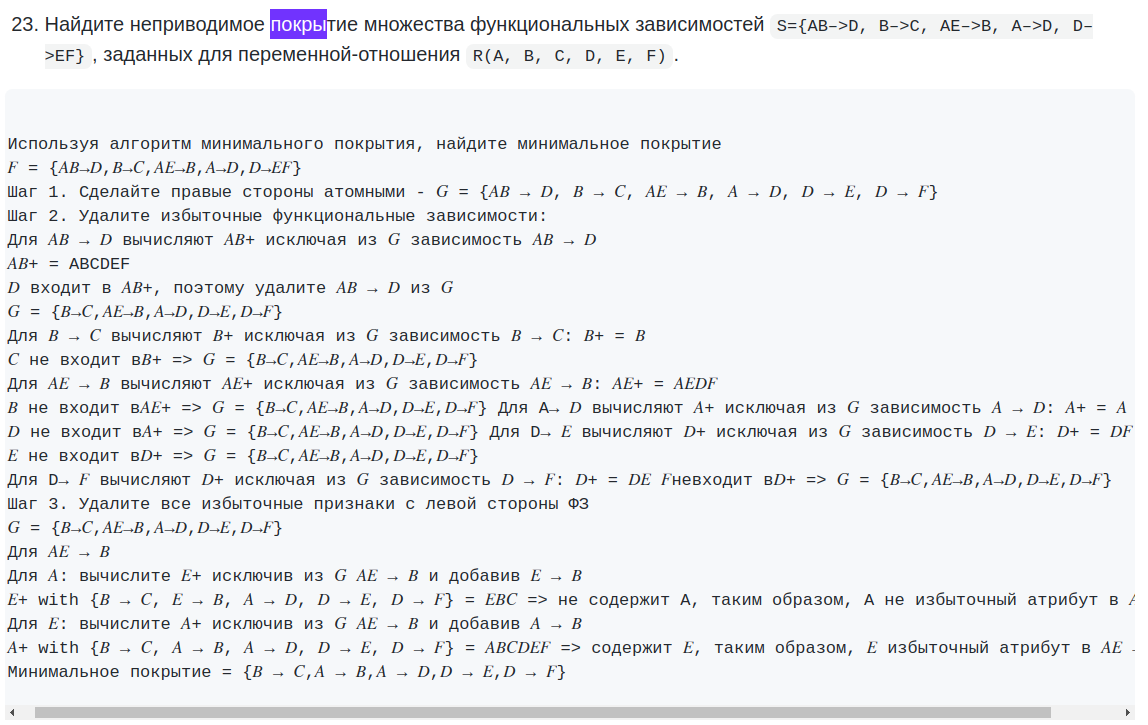
\includegraphics[width=1\textwidth]{04.png}
		\caption{SQL}}
\end{figure}



3. \textbf{Эквивалентность}

Два множества ФЗ S1 и S2 явл эквивалентными тогда и только
тогда когда они явл. покрытиями друг друга.

Есть F - Набор ФЗ.

% $R_F$ = \{A, C, D, E, H\}

% $R_G$ = \{A, C, D, E, H\}

F = \{

A --> C,

AC --> D,

E --> AD,

E --> H

\}

G = \{

A --> CD,

E --> AH

\}

Задача: Доказать что они явл. эквивалентными (или не явл.)

Решение:

1. Проверим G покрывает F?

Найдем замыкание для каждой зависимой части (левой) из G:

\{A\}+ = {A, C, D} (Строим по F)

\{E\}+ = \{E, A, D, H, C\}(Строим по F) = \{E, A, D, H, C\}(Множества
совпадают, значит G покрывает F)

1. Проверим F покрывает G?

Найдем замыкание для каждой зависимой части (левой) из F:

\{A\}+ = \{A, C, D\} (Строим по G)

\{AC\}+ = \{A, C, D\} (Строим по G)

\{E\}+ = \{E, A, H, C, D\} (Строим по G) = \{E, A, H, C, D\}


4. \textbf{Поиск потенциального ключа} (90\%) / суперключа / всех ключей.

Потенциальный ключ (их мб несколько) является не избыточным (Нельзя что-то удалить).

Супер ключ (их мб несколько) - это потенциальный ключ с доп. атрибутами. (не всегда явл супер ключом)

Супер ключ - Супер ключ R - множество атрибутов R, котор.
содержит в виде подмножества хотя бы один (не обязательно соб-
ственный) потенциальный ключ.

\textbf{1. Найти все возможные ключи:}

Схема отношений

R(A, B, C, D, E)

Набор ФЗ:

S = \{A --> C, B --> D, C --> E, E --> A\}

Чтобы найти все возможные ключи перечисляем наборы атрибутов.

\{A, B, C, D, E\}+ = \{A, B, C, D, E\}+ \textbf{Супер ключ}

Проверяем, можно ли удалить какой-то атрибут:

\textbf{1.} \{A, B, C, D\}+ = \{A, B, C, D, E\} (Т.к. == R, то это \textbf{Супер ключ}.
Можно обойтись без E. Т.е. E - не явл. ключевым атрибутом.)

\{A, B, C\}+ = \{A, B, C, D, E\} \textbf{Супер ключ} (Аналогично) (D - лишнее)

\{A, B\}+ = \{A, B, C, D, E\} \textbf{Супер ключ и потенциальный ключ} (Аналогично) (CS - лишнее)

\{A\}+ = \{A, C, E\}+ \textbf{} (Это не полный набор нашей схемы.
B - обязательно ) - не ключ

\{B\}+ = \{B, D\}+ \textbf{} (Аналогично. A - обязательно ) - не ключ.

\textbf{2.}  \{A, B, C, E\}+ = \{A, B, C, E, D\} \textbf{Супер ключ}

\{A, B, E\}+ = \{A, B, E, C, D\}+ \textbf{Супер ключ}

\{A, E\}+ = \{A, E, C\}+ -  (Это не полный набор нашей схемы.
C - обязательно ) - не ключ

\{B, E\}+ = \{B, E, D, A, C\}+  \textbf{Супер ключ и потенциальный ключ}

\{B\}+ = \{B, D\}+ - Не ключ

\{E\}+ =  \{E, A, C\}+ - Не ключ.

И также продолжаем по аналогии\dots

\textbf{3}. \{A, B, D, E\}+ = \dots

\textbf{4}. \{A, C, D, E\}+ = \dots

\textbf{5}. \{B, C, D, E\}+ = \dots

\textbf{1. Найти потенциальные ключи:}

R(A, B, C, D, E)

S = \{A --> B, BC --> E, ED --> A\}

Атрибуты, встречающиеся только в левой части: C,D – (входят во все потенциальные ключи).

Атрибуты, встречающиеся только в правой части: - (не входят в потенциальные ключи).

Атрибуты, не вошедшие в первые 2 группы (которые встречаются и там и там): A, B, E.

\{C,D,A\}+ = \{C,D,A,B,E\} - \textbf{Потенциальный ключ}

Проверка:

\{D,A\}+ = \{D, A, B\}

\{C,A\}+ = \{C,A,B,E\}

\{D,A\}+ = \{D,A,B,\}

\{C,D,B\}+ = \{C,D,A,B,E,A\}- \textbf{Потенциальный ключ}

Проверка: \dots

\{C,D,E\}+ = \{C,D,A,B,E,A\} - \textbf{Потенциальный ключ}

Проверка: \dots



5. \textbf{Выводимость зависимости (да / нет)}

Отношение:

R(A,B,C,D,E,F)

Заданы функциональные зависимости:

S = \{

A --> BC,

B --> E,

CD --> EF

\}

Задача: AD->F Выводимо?

Решение:

\begin{enumerate}
	\item A --> BC => A --> B, A --> C
	\item A --> C => AD --> CD
	\item AD --> CD, CD --> EF => AD --> EF
	\item AD --> EF => AD --> E, AD --> F
\end{enumerate}





